\chapter{Results and Analysis}

    \section{Introduction}
    This chapter provides an overview of the methodology used in the evaluation
    of the implementation of the Roll Call \footnote{a short video demonstration of the Roll
    Call implementation is available at \cite{rc_demo}} and Route-to-Zero protocols. In addition to this, the
    results from a medium scale evaluation are shown and
    discussed.

    \section{Evaluation Methodology}
    The network topology used for the evaluation is a three by four grid with
    a root and nine user nodes as illustrated in figure \ref{fig:test_topology}. With this
    topology, the implementation can be tested with a hop count of three. A single hop
    is the maximum distance a node can broadcast data. From experiments with
    the nRF51 we discovered a hop distance of 4.32m when using a transmission
    power of -30 dBm (minimum transmission power of the nRF51).

    For this experiment the root node sends the RREQs alphabetically, beginning with
    node A and ending with node I.

    \FloatBarrier
    \begin{figure}[ht]
      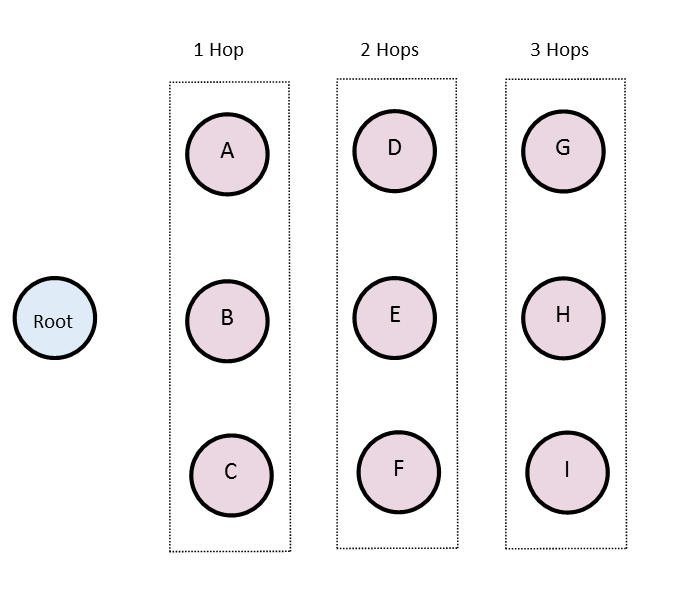
\includegraphics[scale=0.75]{Images/chapter5/setup.png}
      \caption{Evaluation network topology}
      \label{fig:test_topology}
    \end{figure}
    \FloatBarrier

    The metrics measured include:
    \begin{itemize}
      \item Node discovery rate.
            This is the rate at which nodes are discovered, measured from the
            beginning of the protocol until the final node has been identified.
            For the purpose of this experiment, the Route-to-Zero implementation
            knew the total number of nodes in the network.
      \item Total packets sent/processed per node.
            This is the total number of RREQ and RREP packets that are sent
            and processed by each node. Repeat packets are not processed.
      \item Average packets sent/processed per hop.
            This is the average number of packets sent and processed for each hop
            away from the root that a node is. Nodes A, B, and C are one hop away, nodes
            D, E, and F are two hops away, and nodes G, H, and I are three hops away.
    \end{itemize}

    These metrics were recorded using a statistics packet. This packet is sent
    to the root node in the same manner as a RREP packet. This packet contains
    the number of RREQs and RREPS that were received, sent, and processed by
    the node (repeat packets are not counted towards processed packet count).
    For the purpose of this experiment, all statistic packets were sent twenty
    seconds after the receipt of the first RREQ.

    \section{Medium Scale Evaluation Results}

    \subsection{Evaluation Settings}
    The BLE settings used in this experiment are as follows:
    \begin{itemize}
      \item Advertisement Interval: 100ms
      \item Advertisement Period: 500ms
      \item Scan Interval: 50ms
      \item Scan Window: 20ms
    \end{itemize}

    \subsection{Node discovery rate}
    The graph in figure \ref{fig:dsc_rate} shows the number of nodes that were
    discovered with respect to time.

    \FloatBarrier
    \begin{figure}[ht]
      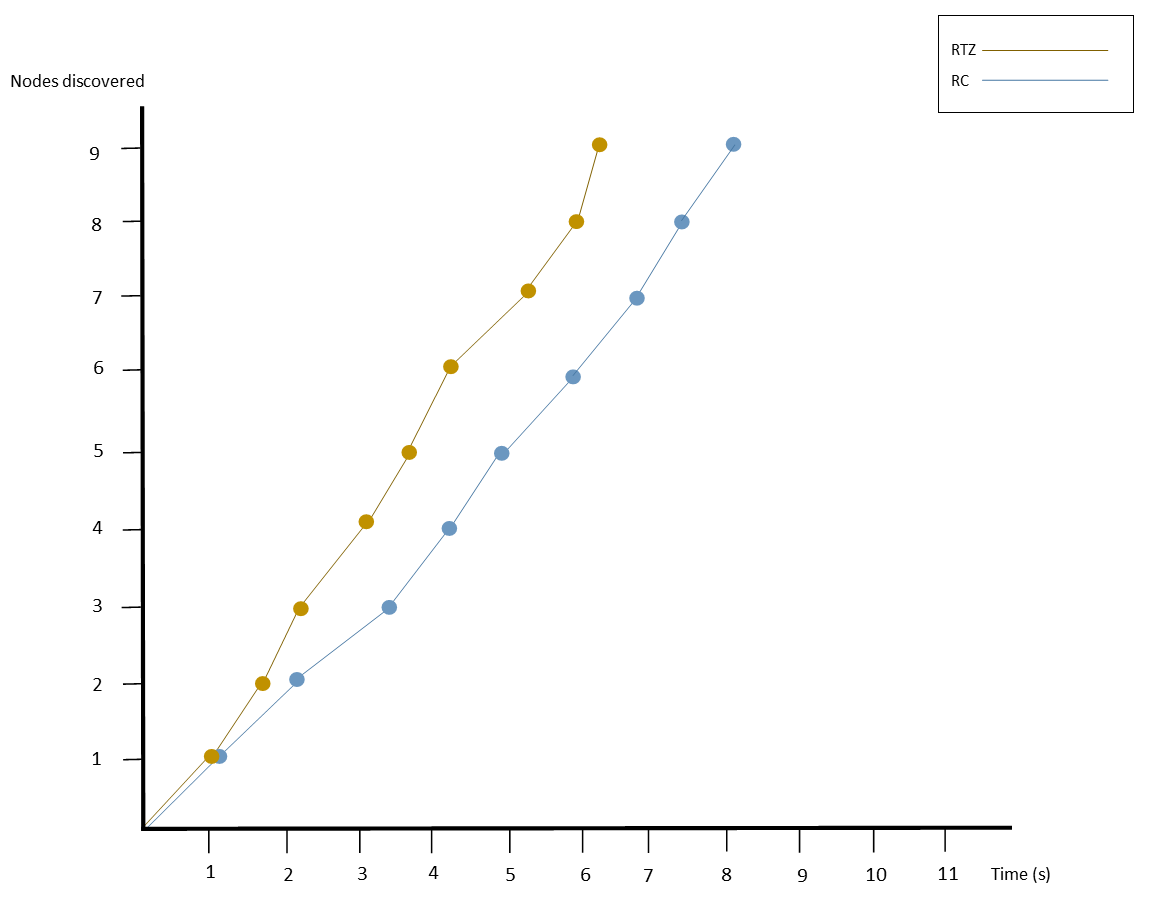
\includegraphics[width=\textwidth]{Images/chapter5/dsc_rate.png}
      \caption{Number of nodes discovered vs time}
      \label{fig:dsc_rate}
    \end{figure}
    \FloatBarrier

    Roll Call (RC) has a discovery rate of 1.06 nodes per second while Rout-to-Zero (RTZ)
    has a discovery rate of 1.34 nodes per second. The reason why RTZ has an improved
    discovery rate is that only a single RREQ is flooded through the network initially,
    meaning that nodes in the first hop can each send their own RREP after forwarding
    the RREQ, and as the wake-up RREQ arrives at subsequent hops, these nodes will
    have already performed a large chunk of the RREQ forwarding from other nodes
    and will we able to send their RREPs sooner than those in RC. In RC, the last
    RREQ from the root is only sent after 4.5 seconds (500ms per RREQ and 9 nodes),
    so when a RREQ arrives at its destination, the node will have its buffer filled
    with other messages to forward and so won't be able to respond with its own
    RREP as quickly. One important thing to note in this scenario is that when
    all nodes are discovered in RC no more packets will be broadcast within the network,
    whereas in RTZ, there may be RREP messages from the root still propagating
    through the network.

    \subsection{Packets per node}
    The graph in figure \ref{fig:pkts_node} shows the number of packets sent
    and processed at each node in the network.

    \FloatBarrier
    \begin{figure}[ht]
      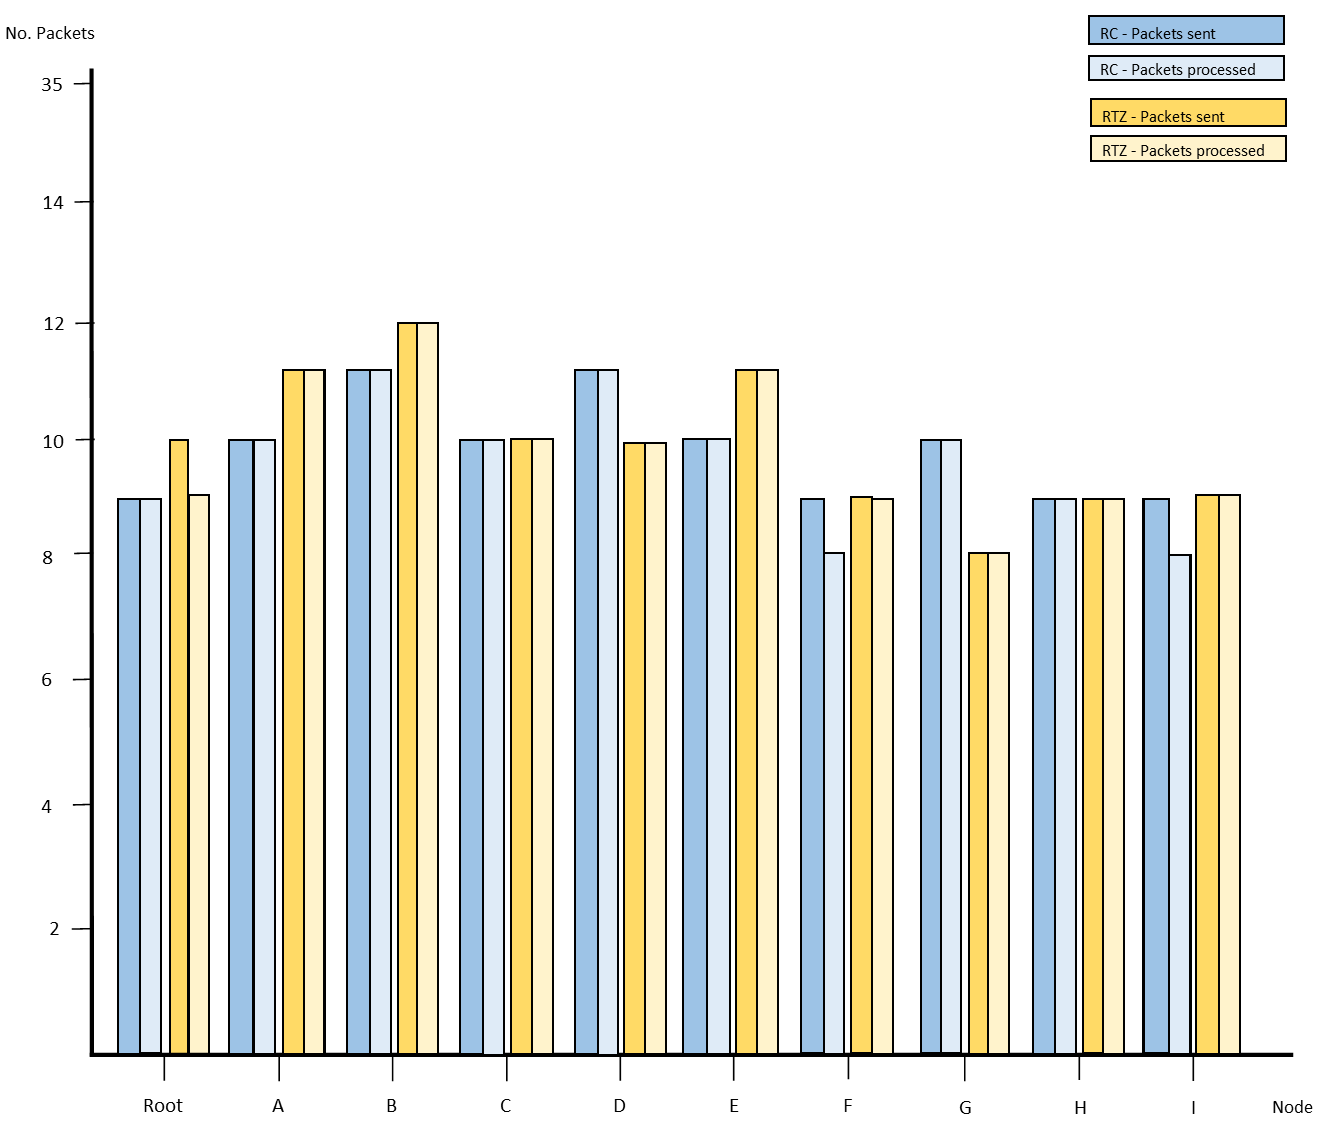
\includegraphics[width=\textwidth]{Images/chapter5/pkts_node.png}
      \caption{Total packets sent/received per node}
      \label{fig:pkts_node}
    \end{figure}
    \FloatBarrier

    The number of packets sent and processed at each node is very similar in both
    protocols and the number of sent packets is largely the same as the number of
    processed packets at each node.
    The reason for this is that if a RREQ is processed, it is either forwarded or a
    RREP is returned. If a RREP is processed, it will be forwarded as RREPs are
    only processed by nodes in the RREP route.

    The network will be flooded with
    repeat packets and broadcasted RREPs due to the nature of BLE advertising, but these packets will not
    have much impact on nodes as they are instantly discarded if repeated or not
    relevant.

    \subsection{Packets per hop}
    The graph in figure \ref{fig:pkts_hop} shows the average number of packets sent
    and received for nodes at different hop counts from the root.

    \FloatBarrier
    \begin{figure}[ht]
      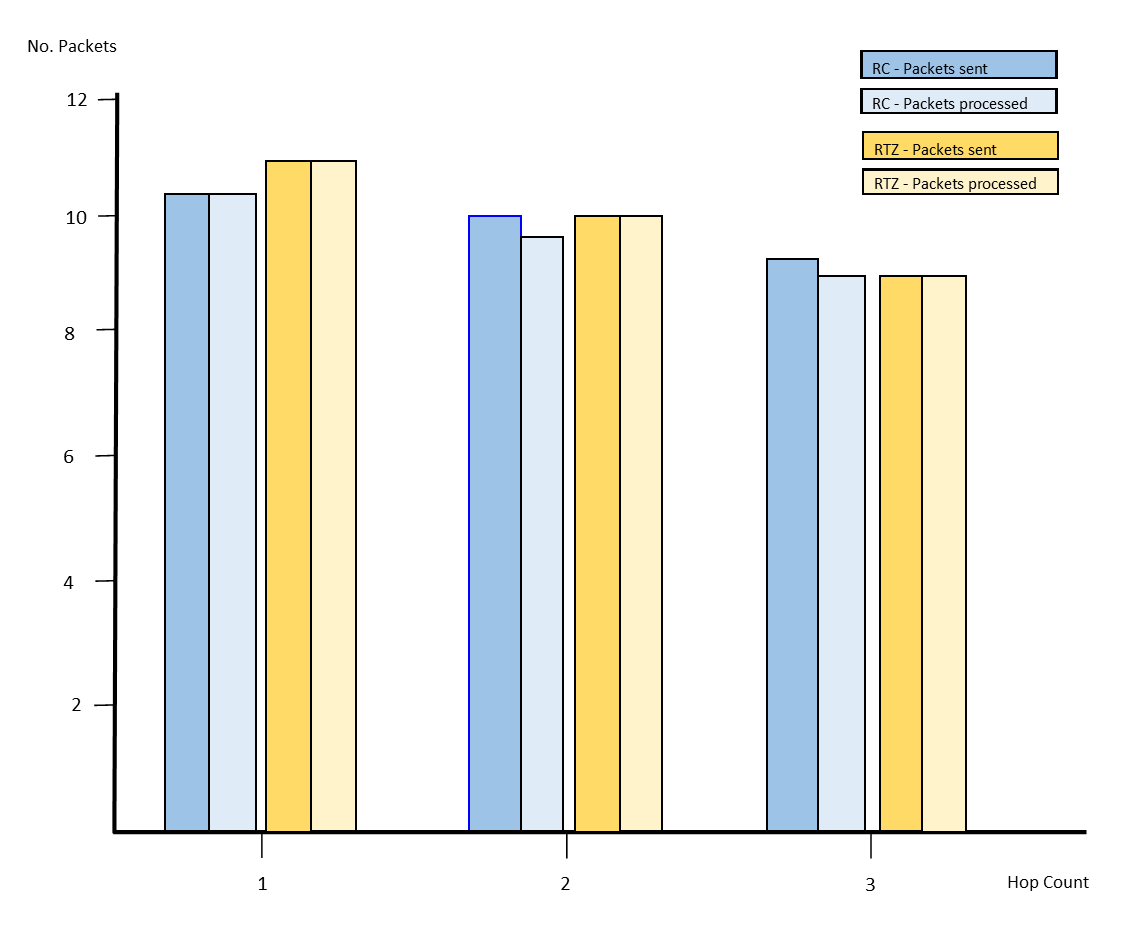
\includegraphics[width=\textwidth]{Images/chapter5/pkts_hop.png}
      \caption{Average packets sent/received vs hops from root}
      \label{fig:pkts_hop}
    \end{figure}
    \FloatBarrier

    The number of packets sent and received increases marginally the closer a node is to
    the root node. The reason for this is that nodes three hops away will not generally
    have any RREPs broadcast to them, so any that are scanned will likely be discarded and
    as a result, throughout the lifetime of the protocol the node will not have to forward any
    RREP packets. With an increased number of hops, and devices further apart, I
    expect this would result in more noticeable differences between hops.

    A difference in packet processing implies that nodes closer to the root consume more power than farther
    nodes as they are advertising for longer periods (if a node has no packets
    in its buffer advertising is turned off). This would only come into effect
    in networks with many more nodes than are present in this network. Nodes 1 hop from the root
    only advertise for \textasciitilde1s longer than those that are 3 hops away.
